\documentclass[a4paper]{article}
\usepackage[T1,T2A]{fontenc}
\usepackage[utf8]{inputenc}
\usepackage[russian]{babel}
\usepackage{amsmath,amssymb}
\usepackage{lmodern}
\usepackage{amssymb,amsmath,mathrsfs,amsthm}
\usepackage{graphicx}
\usepackage{amsthm}
\graphicspath{ {images/} }
\begin{document}
\title{Отчет о проделанной работе за последнее время}

\maketitle 
В последние две недели, как я и говорил, я начал заниматься подготовкой к хакатону deepHack.RL http://rl.deephack.me 

Там нужно было сначала(для попадания на очную часть хакатона) решит задачку типа RL решения для одной игры Atari.
Особенно никто этого делать не умеет, но несколько команд, в том числе наша, смогли предоставить хоть какое-то решение. Игра предлагалась вот такая:
\begin{center}
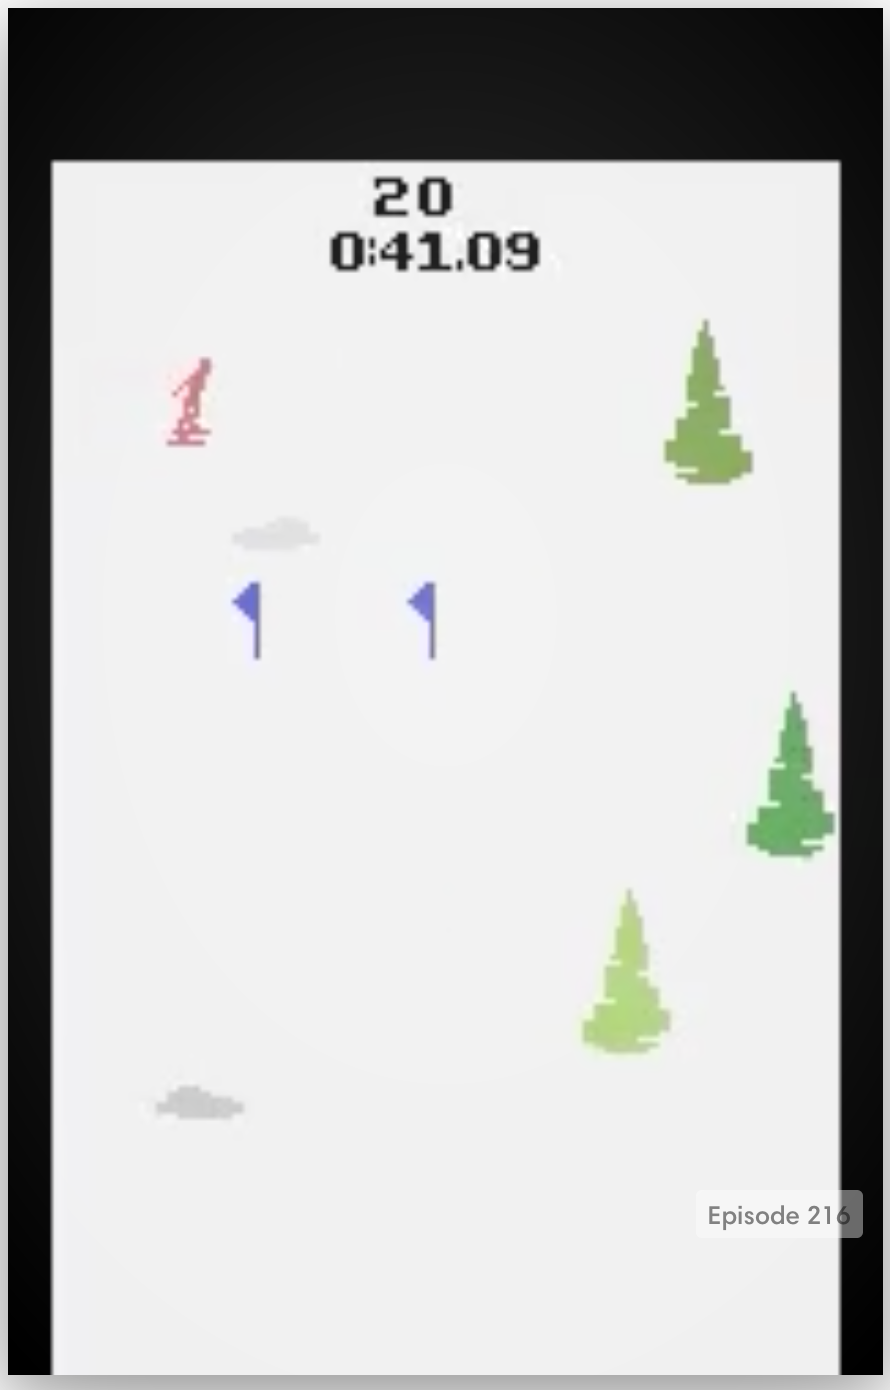
\includegraphics[scale=.3]{skiing}
\end{center} 
Задача в том, чтобы попадать в ворота и спускаться как можно быстрее.
На вход, в качетсве состояния, агенту подается только картинка вроде этой. Нужно было научиться им управлять, но, повторюсь, никто особенно этого так и не научился.

Я решил начать с более простой задачи обучения сетей в RL, но по сути что-то похожее:
\begin{center}
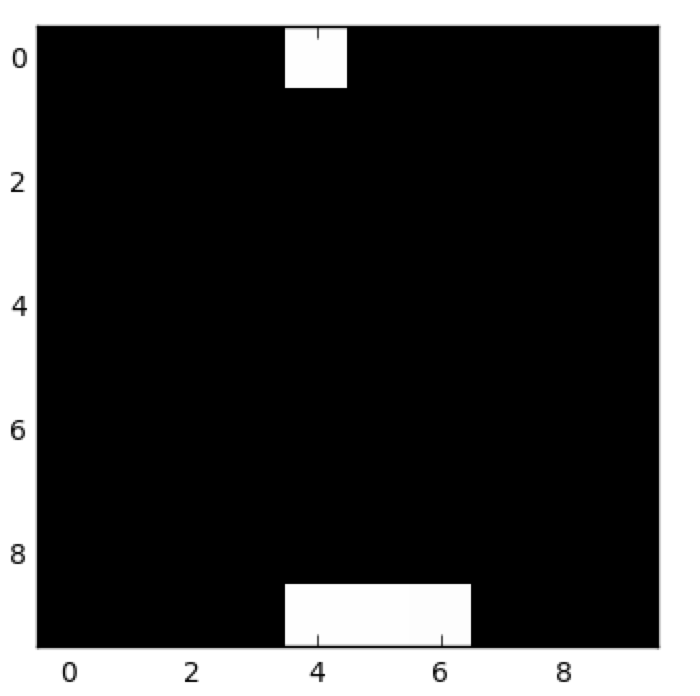
\includegraphics[scale=0.5]{myGame}
\end{center} 
Тут в качествк состояния агент получает черно-белую картинку (никаких оттенков серого, только черный и белый цвет) и должен научится ловить падающий вертикально пиксель при помощи "корзинки" снизу. 
Эта задача намнго проще и поэтому ее удалось решить сразу для размеров 10x10, 20x20, 30x30, вот история обучения алгоритма:

Случай 10x10, уже меньше, чем за 2000 эпизодов сеть обучиласть нормально. По оси y - процент удачных попыток поймать пиксель (0.9 - это лучшее, но что мы надеемся, потому что остальные 10 процентов мы оставили для случайных действий для исследования среды), по х - количетсво эпизодов обучения.
\begin{center}
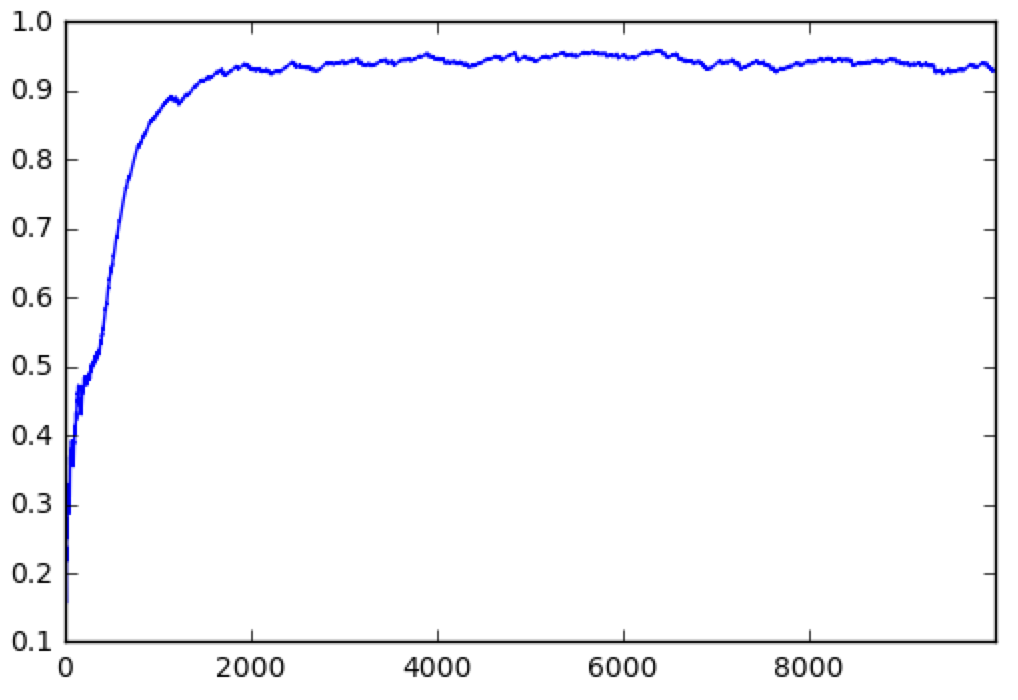
\includegraphics[scale=0.5]{perf10}
\end{center} 
Случай 20x20, тут число эпизодов нужно делить на 20, это связано с моим багом, но я уже не мог перегенерить картинку, потому что процесс обучения достаточно долгий. В общем, чуть меньше, чем за 5000 эпизодов сеть удалось обучить.
\begin{center}
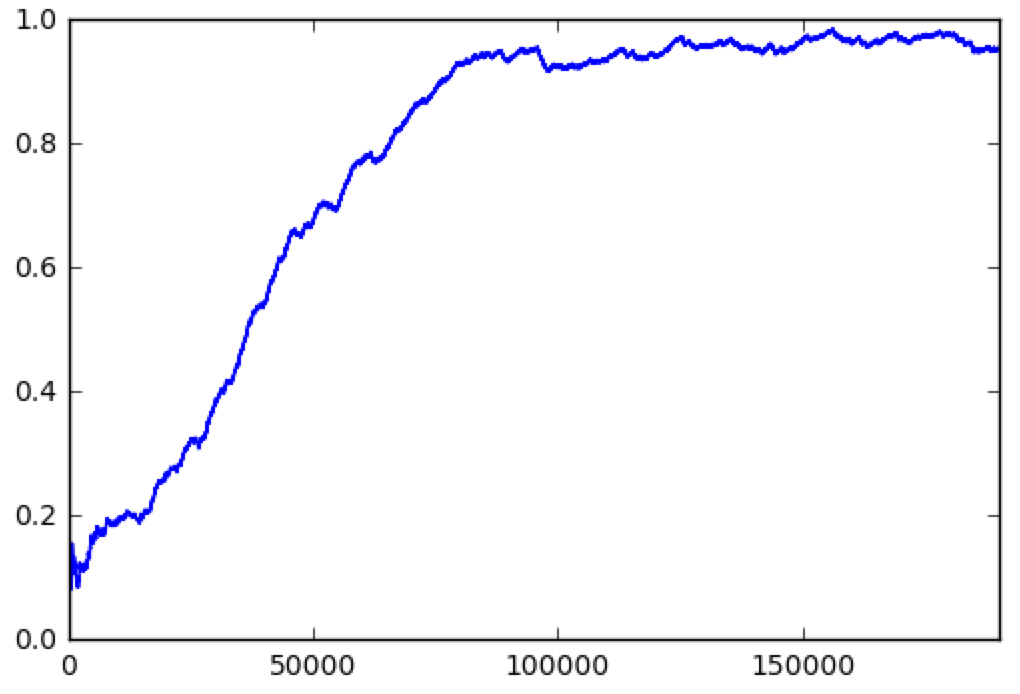
\includegraphics[scale=0.5]{perf20}
\end{center} 
Случай 30x30, тут портебовалось уже больше 15 000 эпизодов для обучения сети.
\begin{center}
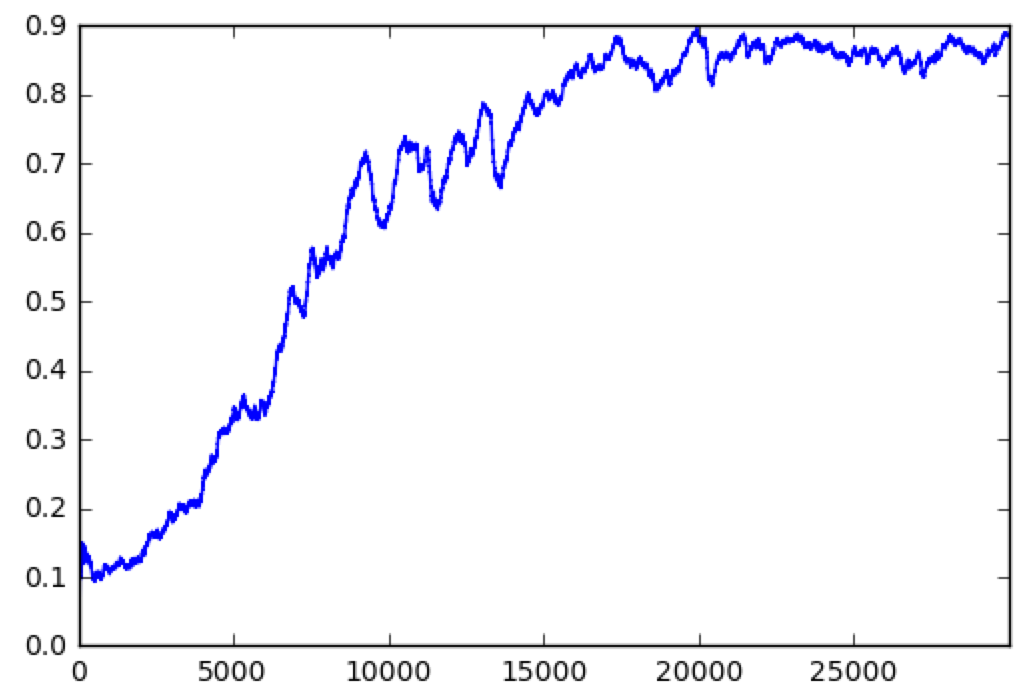
\includegraphics[scale=0.5]{perf30}
\end{center} 

Игру размером 40х40 и больше мне не удалось обучить вовсе, хотя я долго пробовал менять разные конфигурации сети. 

Стоить заметить, что в предыдущих случаях использовалась обычная feed forward сеть, которая запоминает практически все случае отдельно(мне так кажется). 
Я пробовал обучать сверточную сеть, так как она может выделять признаки все более и более общие от слоя к слою. Кажется, что это как раз то, что нам нужно, потому что на первых этапах как раз достоточно знать, что писель где-то в левых 10ти пикселях. А потом уже можно было бы как-то это дальше уточнять.
Это очень важно в больших задачах, чтобы получить хорошее обобщение и не выучивать все отдельные случаи.

Но, повторюсь, обучить сверточную сеть мне пока не удалось даже для сравнительно небольшой задачи (20х20).


В ближайшее время мне хотелось бы научится обучать сверточные сети хотя бы для этой простой задачи и решить ее для размеров 40x40 и 50х50, заодно поработаю над обучением нейронных сетей в целом, благо на работе нам выделели сервер с GPU картами и дают ими пользоваться достаточно свободно.
$$
	Loss(X_{pred}, X_{real}) = - \log	P(\xi = X_{real}), 	
$$

$$
	\xi \sim Poiss(X_{pred}) 
$$
\end{document}